\chapter*{ПРИЛОЖЕНИЯ}
\addcontentsline{toc}{chapter}{ПРИЛОЖЕНИЯ}
\section*{Приложение А}\label{sec:applic_a}
\addcontentsline{toc}{section}{Приложение A}
Здесь приводится подробное описание алгоритма исследования структуры локальных оптимумов. Для удобства изложения, алгоритм разбит
на процедуры: <<Одномерный поиск>>, <<Градиентный подъем>> и <<Исследование локальных оптимумов>>.
\\ \\
\noindent{\textbf{ 1. Одномерный поиск.}}

\noindent{\textbf{ Дано:}}
\begin{itemize}
  \item вектор начального решения $\textbf{x}$ размерности $2N$,
  \item вектор направления одномерного поиска $\textbf{d}$ размерности $2N$,
  \item точность вычислений $\epsilon_{1dim}$.
\end{itemize}
\noindent{\textbf{ Требуется:}} найти вектор $\textbf{x}' = \textbf{x} + \gamma \textbf{d}$ такой, что
\begin{itemize}
  \item $\tilde{F}(\textbf{x}) < \tilde{F}(\textbf{x}'),$
  \item $\tilde{F}(\textbf{x} + (\gamma + \epsilon_{1dim}) \textbf{d}) < \tilde{F}(\textbf{x}').$
\end{itemize}
\begin{enumerate}
  \item Инициализировать параметр одномерного поиска $\beta := 1$, вектор $\textbf{x}' := \textbf{x}$, счетчик итераций $j := 1$.
  \item Если $\tilde{F}(\textbf{x}' + \beta \textbf{d}) < \tilde{F}(\textbf{x}')$, то уменьшить $\beta := \beta / 2$.
  В противном случае, в зависимости от значения счетчика:\\
  при $j = 1$ положить $\textbf{x}_a := \textbf{x}'$,\\
  при $j = 2$ положить $\textbf{x}_b := \textbf{x}'$,\\
  при $j = 3$ положить $\textbf{x}_c := \textbf{x}'$,\\
  при $j > 3$ положить $\textbf{x}_a := \textbf{x}_b$, $\textbf{x}_b := \textbf{x}_c$, $\textbf{x}_c := \textbf{x}'$.\\
  При этом, вне зависимости от значений счетчика, $\beta := 2\beta$,\\
  $\textbf{x}' := \textbf{x}' + \beta \textbf{d}.$
  \item Если $\beta < \epsilon_{1dim}$ и $j < 3$, вернуть $\textbf{x}'$.
  \item Если $\beta < \epsilon_{1dim}$ и $j \geq 3$, то переходим к шагу 5, иначе - на шаг 2.
  \item По точкам $\textbf{x}_a, \textbf{x}_b, \textbf{x}_c$ строим квадратичную аппроксимацию:
   $$\textbf{x}^{*} := (\textbf{x}_b - 3 \beta \textbf{d}) +
   \left(\beta\left(1 + \frac{\tilde{F}(\textbf{x}_a) - \tilde{F}(\textbf{x}_c)}{2(\tilde{F}(\textbf{x}_a) -
   2\tilde{F}(\textbf{x}_b) + \tilde{F}(\textbf{x}_c))}\right)\right)\textbf{d}.$$\\
\end{enumerate}
{ \textbf{2. Градиентный подъем.}}
\\ \\
\noindent{\textbf{Дано:}}
\begin{itemize}
  \item вектор начального решения $\textbf{x}_0$ размерности $2N$,
  \item точность вычислений $\epsilon_{grad}$,
  \item точность вычислений одномерного поиска $\epsilon_{1dim}$,
  \item время принудительного завершения работы алгоритма $time_{finish}.$\\
\end{itemize}
\noindent{\textbf{Требуется:}} найти вектор $\textbf{x}$ такой, что
для всех $$\textbf{d}, |\textbf{d}| = 1 \text{~выполняется~} \tilde{F}(\textbf{x} + (\epsilon_{grad})\textbf{d}) < \tilde{F}(\textbf{x})$$.\\
\begin{enumerate}
  \item $\textbf{x} := \textbf{x}_0.$
  \item Вычислить и нормировать градиент целевой функции:
   $$\textbf{d} := \frac{\nabla \tilde{F}(\textbf{x})}{|\nabla \tilde{F}(\textbf{x})|}.$$
  \item Вычислить $\textbf{x}^{*}$ алгоритмом одномерного поиска~1 с параметрами $\textbf{x}, \textbf{d}, \epsilon_{1dim}.$
  \item Записать в $time$ текущее время. Если $time \geq time_{finish}$, вернуть $\textbf{x}^{*}$.
  \item Если $|\tilde{F}(\textbf{x}) - \tilde{F}(\textbf{x}^{*})| < \epsilon_{grad}$, вернуть $\textbf{x}^{*}$, иначе положить $\textbf{x} = \textbf{x}^{*}$ и повторить~шаги~2-5.\\ \\
\end{enumerate}

\noindent{\textbf{ 3. Исследование локальных оптимумов.}}
\\ \\
\noindent{\textbf{Дано:}}
\begin{itemize}
  \item $x_{\max}$ как верхняя оценка нормы допустимой области,
  \item точность вычислений $\epsilon_{grad}$,
  \item точность вычислений одномерного поиска $\epsilon_{1dim}$,
  \item время принудительного завершения работы алгоритма $time_{finish}$,
  \item максимально допустимая норма вектора ${\textbf{y}}$, обозначаемая за ${\textbf{y}}_{\max}$.\\
\end{itemize}

\noindent{\textbf{Требуется:}} провести исследование структуры локальных оптимумов, как описано в разделе~\ref{sec:exp}.\\

\begin{enumerate}
  \item Инициализировать каждую компоненту начального вектора $x_{0,i = \overline{1,2N}}$ равномерно распределенной в интервале $[-x_{\max}, x_{\max}]$
  величиной.
  \item Вычисляем допустимый вектор $\textbf{x}$ путем масштабирования $\textbf{x}_0$ в допустимую область:
  $$\textbf{x} := (\max_{k=\overline{1,n}} {\textbf{x}_0}^T \textbf{H}^{(k)}{\textbf{x}_0})^{-1/2} {\textbf{x}_0}.$$
  \item Вычислить ${\textbf{x}^{*}}$ алгоритмом градиентного подъема~(2) с параметрами ${\textbf{x}}, \epsilon_{grad}, \epsilon_{1dim}, time_{finish}.$
  \item Записать в $time$ текущее время. Если $time$ < $time_{finish}$, перейти на шаг~1.
  \item Для каждого найденного решения установить ${\textbf{x}_0^{*}} = {\textbf{x}^{*}}$, составить линеаризованную задачу~(\ref{eq:task5}) и найти
  ее решение ${\textbf{x}_{lp}^{*}}$.
  \item Исключить решения, для которых $|{\textbf{x}_0^{*}} - {\textbf{x}_{lp}^{*}}| > {\textbf{y}_{\max}}$. В случае оставшихся решений установить
  $\textbf{x} = {\textbf{x}_{lp}^{*}}$ и повторить шаги~2-3. Оценить норму разницы $|{\textbf{x}_0^{*}} - {\textbf{x}^{*}}|$. Вернуть ${\textbf{x}_0^{*}}$ с
  лучшим значением $\tilde{F}({\textbf{x}_0^{*}})$ в качестве результата.
\end{enumerate}

\section*{Приложение Б}
\addcontentsline{toc}{section}{Приложение Б}
\label{sec:applic_b}
Комплекс моделирования и решения задач оптимизации направленности ФАР КВ диапазона <<Expi>> предназначен для моделирования антенных систем и вычисления управляющих параметров фазированных антенных решеток (ФАР).Регистрируемая программа для ЭВМ применима в радиотехнике
при оптимизации направленного излучения ФАР КВ диапазона.Программа позволяет запускать файлы заданного формата с инструкциями по организации вычислительного эксперимента, редактировать их, визуализировать результаты.
Здесь приводится графический интерфейс и функциональные возможности разработанного в рамках текущей работы программного комплекса <<Expi>>.

\subsection*{Графический интерфейс}
  Программное окно разделено на три части: обозреватель текущей директории, окно вывода и рабочая область. Содержимое рабочей области меняется, в зависимости от выбранного файла. В случае, если выбран файл эксперимента~(.exp), оно представляет собой редактор текстового файла~(рис.~(\ref{ic:applic_b_edit})). Для файла формата .nec будет представлен обозреватель геометрии антенной системы~(рис.~(\ref{ic:applic_b_preview})), Для файлов формата .svg, в которые производится запись диаграмм направленности, приводится предпросмотр данного графического формата~(рис.~(\ref{ic:applic_b_results})).

\begin{figure}[h!]
  \centering
  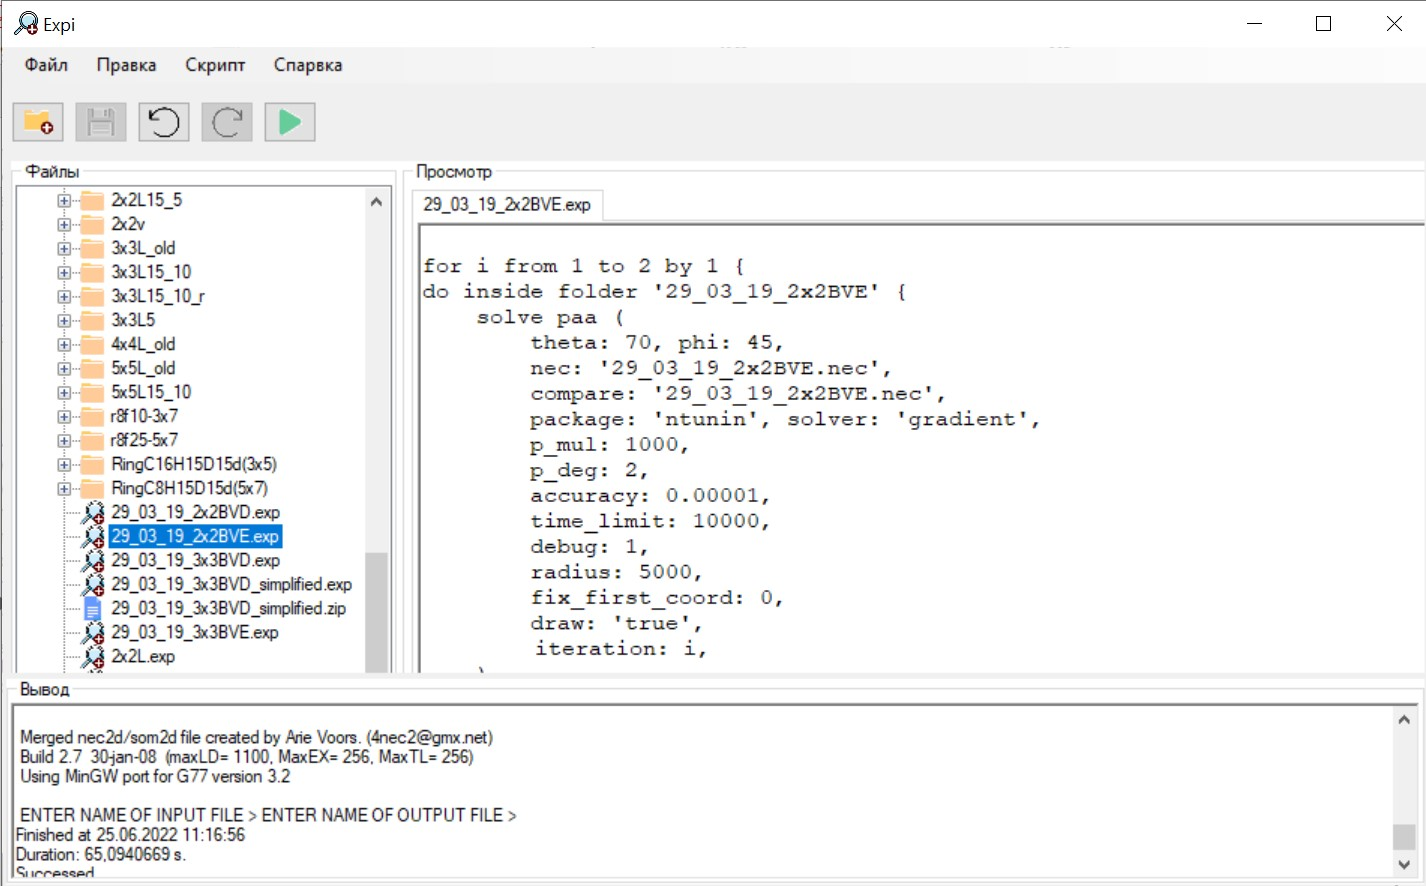
\includegraphics[width=\linewidth]{expi_script.jpeg}
  \caption{Редактор исполняемых файлов}
  \label{ic:applic_b_edit}
\end{figure}

\begin{figure}[h!]
  \centering
  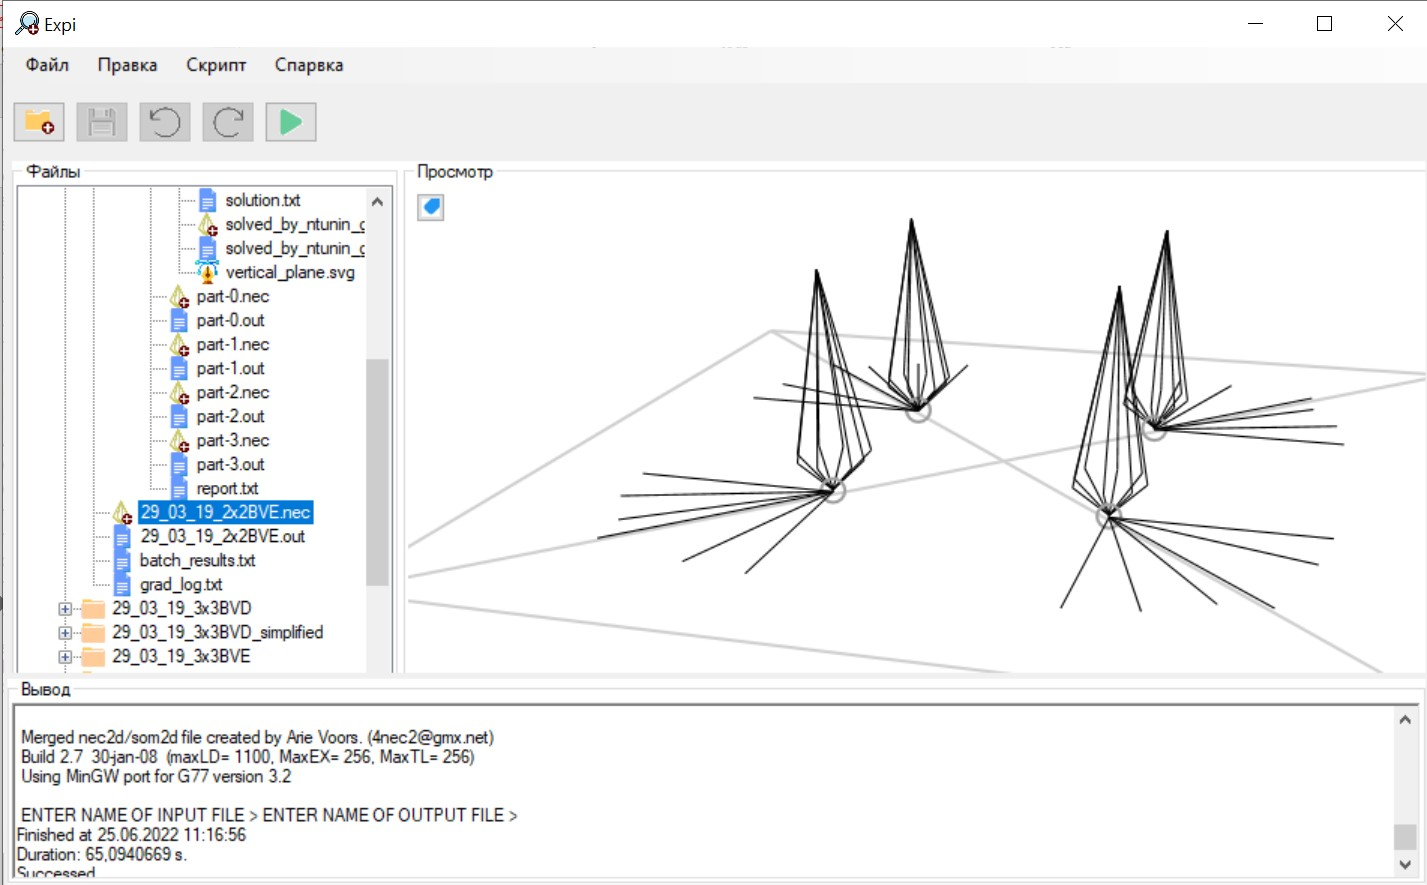
\includegraphics[width=\linewidth]{expi_paa.jpeg}
  \caption{Предпросмотр геометрии}
  \label{ic:applic_b_preview}
\end{figure}

\begin{figure}[h!]
  \centering
  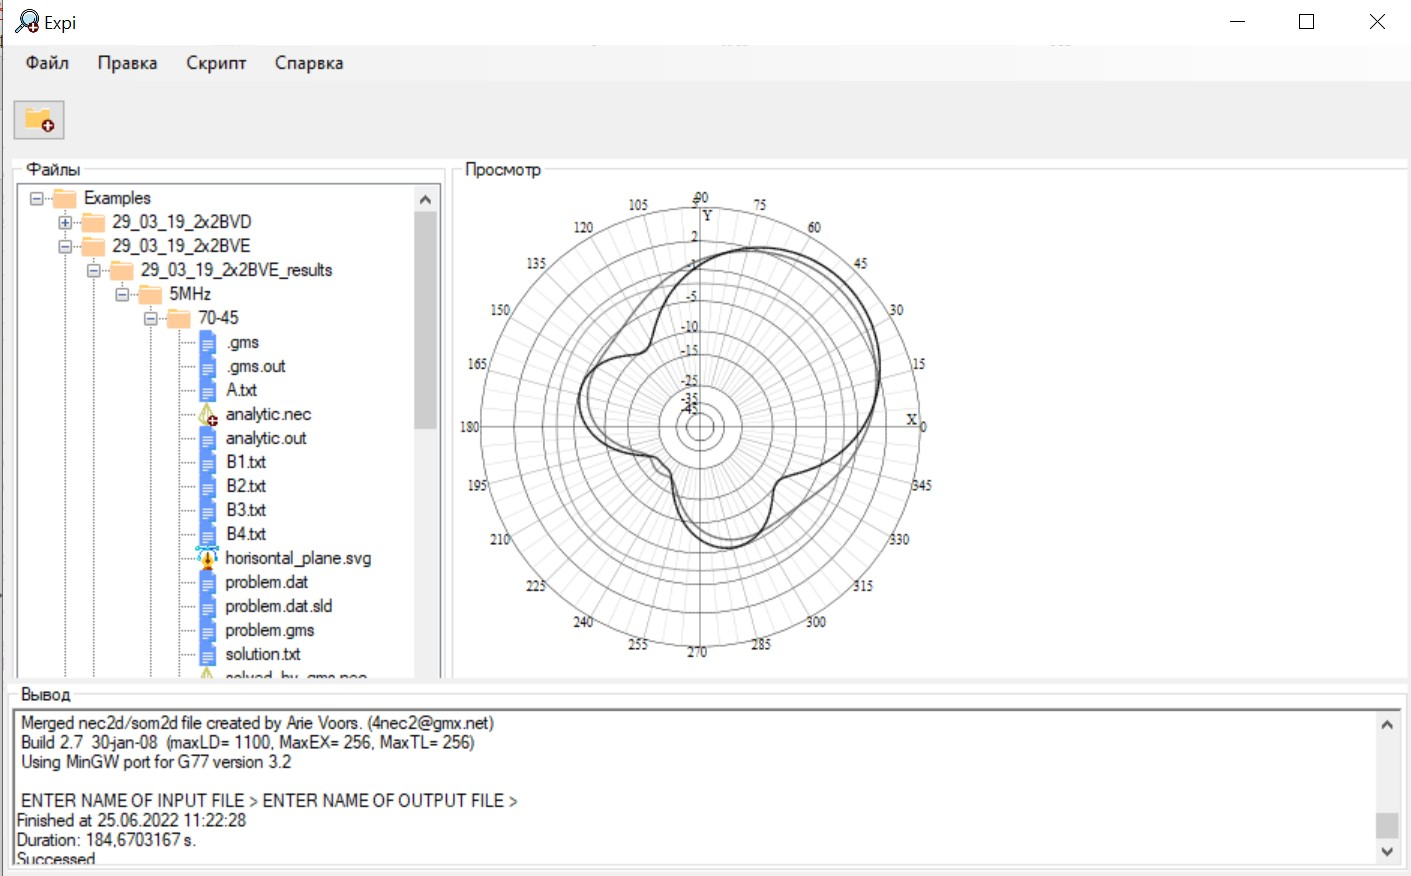
\includegraphics[width=\linewidth]{expi_results.jpeg}
  \caption{Предпросмотр результатов}
  \label{ic:applic_b_results}
\end{figure}

\subsection*{Языковые конструкции}
Комплекс <<Expi>> является, по сути, скриптовым интерпретатором одноименного языка, также разработанного автором в рамках текущей работы. Далее приводятся основные синтаксические конструкции.

\begin{lstlisting}[caption={Переменные}, label={experiment}]
def x = 1
def point = (0, 0, 1)
\end{lstlisting}

\begin{lstlisting}[caption={Сегментированный провод}, label={experiment}]
(0, 0, 0) -> (1, 0, 1) -> (0, 0, 5)
(0, 0, 0) -> (1, 0, 1) ~1v~ (0, 0, 5)
(0, 0, 0) -> (1, 0, 1) ~1+0.5iA~ (0, 0, 5)
\end{lstlisting}

\begin{lstlisting}[caption={Линейные преобразования}, label={experiment}]
translate x to 0.5
translate to (0, 0, 1)
rotate around z by pi/2
\end{lstlisting}

\begin{lstlisting}[caption={Циклы}, label={experiment}]

for angle from 0 to 2 * pi by pi/8 {
   rotate around z by angle
   (0, 0, 0) -> (1, 0, 0)
}

for angle from 0 up to 2 * pi by pi/8 {
   rotate around z by angle
   (0, 0, 0) -> (1, 0, 0)
}

\end{lstlisting}


\begin{lstlisting}[caption={Группы команд}, label={experiment}]
def Emitter {
    for angle from 0 to 2 * pi by pi/8 {
       rotate around z by angle
       (0, 0, 0) -> (1, 0, 0)
    }
}

translate x to -5
Emitter
translate x to 5
Emitter
\end{lstlisting}

\begin{lstlisting}[caption={Оптимизация направленности ФАР}, label={experiment}]
solve paa (
    n: 'bve_2x2.nec',
    theta: 70,
    phi: 45,
    p: 'ntunin',
    s: 'grad',
    c: 'bve.nec',
    p_mul: 1000000,
    p_deg: 4,
    time_limit: 1000,
    accuracy: 0.000001
)
\end{lstlisting}



\begin{lstlisting}[caption={Полный текст примера вычислительного эксперимента}, label={experiment}]

def knees = 8
def height = 15
def kneeWidth = 2.5
def base = 0.5
def rize = 2
def radialsCount = 6
def radialLength = 15
def size = 2
def distance = 20

def Drop {
   def step = 2 * pi / knees
   for angle from 0 to 2 * pi by step {
      rotate around z by angle
      (0, 0, 0) -> (kneeWidth, 0, kneeWidth) -> (0, 0, height)
   }
}

def BVE {
   (0, 0, 0) ~1v~ (0, 0, base)
   def step = pi / 2 / (radialsCount - 1)
   for i from 0 to  radialsCount  by 1 {
       rotate around z by i * step
       (0, 0, 0) -> (radialLength, 0, 0)
   }
   translate z to base
   Drop
}

def PlaceBVE {
   translate to (x, y, 0)
   rotate around z by angle
   BVE
}

def PAA {
   def width = (size - 1) * distance
   def left = -width/2
   def right = width/2
   def top = width/2
   def bottom = -width/2

   PlaceBVE(x: left, y: top, angle: pi / 2)
   PlaceBVE(x: right, y: top, angle: 0)
   PlaceBVE(x: right, y: bottom, angle: -pi / 2)
   PlaceBVE(x: left, y: bottom, angle: pi)
}

def ExportPAA {
    export nec (n: 'bve_${size}x${size}.nec', f: 5, g: 'real') {
        translate z to rize
        PAA
    }
}

def One {
    (0, 0, 0) ~1v~ (0, 0, base)
    def oneRadialsCount = (radialsCount - 1) * 4
    def step = 2 * pi / (oneRadialsCount - 1)
    for i from 0 to  oneRadialsCount by 1 {
        rotate around z by i * step
        (0, 0, 0) -> (radialLength, 0, 0)
    }
    translate z to base
    Drop
}

def ExportOne {
    export nec (n: 'bve.nec', f: 5, g: 'real') {
        translate z to rize
        One
    }
}

do inside folder '05.04.22' {
    ExportOne
    ExportPAA

    solve paa (
        n: 'bve_${size}x${size}.nec',
        theta: 70,
        phi: 45,
        p: 'ntunin',
        s: 'grad',
        c: 'bve.nec',
        p_mul: 1000000,
        p_deg: 4,
        time_limit: 1000,
        accuracy: 0.000001
    )
    solve paa (
        n: 'old_bve_${size}x${size}.nec',
        theta: 70,
        phi: 45,
        p: 'ntunin',
        s: 'grad',
        c: 'bve.nec',
        p_mul: 1000000,
        p_deg: 4,
        time_limit: 1000,
        accuracy: 0.000001
    )
}

\end{lstlisting}

\newpage

\subsection*{Свидетельство о государственной регистрации}

\begin{figure}[!h]
\center{
\includegraphics[width=0.9\linewidth]{expi_reg.jpeg}}
\caption{Свидетельство о государственной регистрации}
\label{ris:expi_reg}
\end{figure} 

\newpage

\section*{Приложение В}\label{sec:applic_c}
\addcontentsline{toc}{section}{Приложение В}
\begin{figure}[!h]
\center{
\includegraphics[width=0.9\linewidth]{education_act.jpeg}}
\label{ris:education_act}
\end{figure} 

\newpage

\fixme{Акт о внедрении в производство (на подписании)}
%\begin{figure}
%\center{
\includegraphics[width=0.95\linewidth]{industry_act.jpeg}}
%\caption{Свидетельство о государственной регистрации}
%\label{ris:industry_act}
%\end{figure} 